%%%%%%%%%%%%%%%%%%%% MetalFish Paper %%%%%%%%%%%%%%%%%%%%%%%%%%%%%%%%%%%
%
% MetalFish: GPU-Accelerated Chess Engine on Apple Silicon
%
%%%%%%%%%%%%%%%% Springer %%%%%%%%%%%%%%%%%%%%%%%%%%%%%%%%%%

\documentclass{svproc}

\usepackage{url}
\def\UrlFont{\rmfamily}
\usepackage{graphicx}
\usepackage{float}
\usepackage{amsmath}
\usepackage{algorithm}
\usepackage{algpseudocode}
\usepackage{booktabs}
\usepackage{listings}
\usepackage{xcolor}
\usepackage{pgfplots}
\pgfplotsset{compat=1.18}

% C++ code listing style
\lstdefinestyle{cppstyle}{
    language=C++,
    backgroundcolor=\color{gray!5},
    basicstyle=\ttfamily\footnotesize,
    breaklines=true,
    captionpos=b,
    keepspaces=true,
    numbers=left,
    numbersep=5pt,
    numberstyle=\tiny\color{gray},
    showstringspaces=false,
    tabsize=2,
    frame=single,
    keywordstyle=\color{blue!70!black},
    commentstyle=\color{green!50!black},
    stringstyle=\color{red!60!black},
    morekeywords={uint64_t, int32_t, int16_t, int8_t, uint, device, kernel, constant, thread_position_in_grid}
}

\begin{document}
\mainmatter

\title{MetalFish: A GPU-Accelerated Chess Engine\\for Apple Silicon Unified Memory Architecture}

\titlerunning{MetalFish: GPU Chess Engine}

\author{Nripesh Niketan\inst{1}}

\authorrunning{N. Niketan}

\institute{Independent Researcher\\
\email{nripesh14@gmail.com}}

\maketitle

\begin{abstract}
We present MetalFish, a hybrid CPU-GPU chess engine implementing Stockfish-style alpha-beta search with Metal GPU acceleration on Apple Silicon unified memory architecture. Our empirical evaluation reveals a fundamental challenge: GPU kernel dispatch overhead (703~$\mu$s median blocking latency) exceeds CPU NNUE evaluation time (84~ns median) by approximately 8,400$\times$ for single positions, making GPU acceleration counterproductive for traditional tree search. This overhead arises from Metal command buffer creation, encoding, and synchronization---inherent costs that cannot be amortized without batching thousands of positions per dispatch. We present detailed measurements including percentile distributions and discuss the architectural implications for GPU-accelerated game engines. The implementation achieves 1.43 million nodes per second using CPU evaluation. Our findings suggest that GPU acceleration for chess engines is most effective when combined with batch-oriented search algorithms such as MCTS, or when true multi-position batching within a single dispatch can be achieved.

\keywords{Chess Engine, GPU Computing, Metal, NNUE, Unified Memory, Apple Silicon}
\end{abstract}

\section{Introduction}

Modern chess engines achieve remarkable playing strength through sophisticated alpha-beta search enhanced with neural network evaluation. Stockfish combines Principal Variation Search (PVS) with Efficiently Updatable Neural Networks (NNUE) to achieve superhuman performance~\cite{Stockfish2024}. The emergence of GPU computing presents opportunities to accelerate evaluation-intensive components, but the sequential dependencies inherent in alpha-beta search create fundamental challenges for GPU parallelization~\cite{Nickolls2008}.

MetalFish investigates these challenges through a hybrid CPU-GPU architecture leveraging Apple Silicon's unified memory. Rather than attempting full GPU parallelization of alpha-beta search, we maintain traditional CPU-based search while implementing GPU kernels for NNUE evaluation. Our empirical results reveal that GPU dispatch overhead dominates single-position workloads, providing concrete guidance for hybrid engine design.

\subsection{Contributions}

This paper makes the following contributions:

\begin{enumerate}
\item An empirical characterization of Metal GPU dispatch overhead showing 703~$\mu$s median blocking latency versus 84~ns for CPU evaluation---an 8,400$\times$ slowdown for single positions.

\item Metal compute kernels for sparse feature transformation and incremental accumulator updates, demonstrating unified memory buffer allocation via \texttt{MTLResourceStorageModeShared}.

\item Analysis of the crossover point: GPU acceleration requires batching approximately 8,400 positions per dispatch to match CPU throughput, making it impractical for traditional alpha-beta search but potentially viable for MCTS or multi-position analysis.

\item A complete, tested implementation achieving 1.43M nodes/second with correct perft results, providing a baseline for future GPU chess engine research.
\end{enumerate}

\section{Background}

\subsection{Alpha-Beta Search}

The minimax algorithm with alpha-beta pruning forms the foundation of modern chess engines~\cite{Knuth1975}. Alpha-beta maintains bounds $[\alpha, \beta]$ representing the range of possible values; when $\alpha \geq \beta$, remaining siblings can be pruned. Principal Variation Search (PVS) refines this by assuming the first move is optimal, searching subsequent moves with zero-width windows~\cite{Reinefeld1983}.

\subsection{NNUE Evaluation}

Efficiently Updatable Neural Networks (NNUE) use a large sparse input layer representing piece-square combinations, followed by smaller dense layers~\cite{Nasu2018}. The key insight is that activations can be updated incrementally as moves are made, rather than recomputing from scratch. Stockfish's NNUE architecture uses:
\begin{itemize}
\item Feature transformer: 45,056 inputs $\rightarrow$ 1,024 hidden units
\item FC0: 2,048 $\rightarrow$ 16 (concatenated perspectives)
\item FC1: 16 $\rightarrow$ 32 with squared clipped ReLU
\item FC2: 32 $\rightarrow$ 1 output score
\end{itemize}

The quantization uses 6-bit right shifts for weight scaling:
\begin{equation}
\text{clipped\_relu}(x) = \min(\max(x \gg 6, 0), 127)
\end{equation}

\subsection{Unified Memory Architecture}

Apple Silicon's unified memory allows CPU and GPU to access the same physical memory coherently~\cite{AppleMetal2024}. Using \texttt{MTLResourceStorageModeShared}, buffers are accessible from both processors without explicit copying, eliminating the traditional discrete GPU bottleneck.

\section{System Architecture}

\subsection{Design Overview}

MetalFish implements three primary components:

\textbf{CPU Search Engine:} Executes complete alpha-beta search including PVS, move ordering via history heuristics, and pruning techniques. All control flow remains on CPU to avoid GPU branch divergence.

\textbf{GPU Evaluation Engine:} Implements NNUE inference through Metal compute shaders for feature transformation and network forward passes.

\textbf{Unified Memory Interface:} Manages shared buffers using \texttt{MTLResourceStorageModeShared}, enabling zero-copy access from both CPU and GPU.

\subsection{Search Implementation}

The search implements Stockfish-style techniques:

\textbf{Move Ordering:} Butterfly history, capture history, continuation history, killer moves, and counter moves.

\textbf{Extensions:} Singular extension with double/triple variants for strongly singular moves; check extension.

\textbf{Pruning:} Null move pruning with verification search, late move reductions, futility pruning, SEE pruning, and ProbCut.

\textbf{Transposition Table:} Zobrist hashing~\cite{Zobrist1970} with depth-preferred replacement and generation aging.

\subsection{GPU NNUE Kernels}

\subsubsection{Feature Transformation}

The feature transformer converts sparse HalfKAv2 features to dense accumulators. Each thread computes one output element:

\begin{lstlisting}[style=cppstyle, caption={Feature transformation kernel}]
kernel void feature_transform(
    device const int16_t* weights,
    device const int16_t* biases,
    device const int* features,
    device int32_t* accumulator,
    constant int& num_features,
    constant int& ft_dims,
    uint h [[thread_position_in_grid]])
{
    if (h >= ft_dims) return;
    int32_t sum = biases[h];
    for (int i = 0; i < num_features; i++) {
        int f = features[i];
        sum += weights[f * ft_dims + h];
    }
    accumulator[h] = sum;
}
\end{lstlisting}

Kernel configuration: 1,024 threads dispatched as a single threadgroup, processing all hidden units in parallel. Memory layout stores weights in feature-major order for coalesced access when multiple threads read the same feature.

\subsubsection{Incremental Updates}

When a move is made, only changed features require updating:

\begin{lstlisting}[style=cppstyle, caption={Incremental accumulator update}]
kernel void feature_update(
    device const int16_t* weights,
    device int32_t* accumulator,
    device const int* added,
    device const int* removed,
    constant int& num_added,
    constant int& num_removed,
    constant int& ft_dims,
    uint h [[thread_position_in_grid]])
{
    if (h >= ft_dims) return;
    int32_t delta = 0;
    for (int i = 0; i < num_added; i++)
        delta += weights[added[i] * ft_dims + h];
    for (int i = 0; i < num_removed; i++)
        delta -= weights[removed[i] * ft_dims + h];
    accumulator[h] += delta;
}
\end{lstlisting}

\subsection{Unified Memory Buffer Allocation}

Buffer allocation uses shared storage mode:

\begin{lstlisting}[style=cppstyle, caption={Shared buffer allocation}]
MTL::ResourceOptions opts = 
    MTL::ResourceStorageModeShared;
ft_weights = device->newBuffer(
    FT_IN_DIMS * FT_OUT_DIMS * sizeof(int16_t),
    opts);
// CPU access: ft_weights->contents()
// GPU access: direct in kernel
\end{lstlisting}

This enables the CPU to write position features and read evaluation results without explicit memory transfers.

\section{Experimental Results}

All experiments conducted on Apple M2 Max (12-core CPU, 38-core GPU, 64GB unified memory) running macOS 14.0, Metal feature set macOS-GPUFamily2-v1.

\subsection{GPU NNUE Implementation}

The GPU NNUE implementation loads both Stockfish networks to GPU memory:

\begin{table}[t]
\caption{GPU NNUE memory allocation on M2 Max}
\label{tab:gpu_mem}
\centering
\begin{tabular}{lrr}
\toprule
Component & Big Network & Small Network \\
\midrule
Feature transformer weights & 45,056 KB & 5,632 KB \\
Feature transformer biases & 2 KB & 0.25 KB \\
PSQT weights & 704 KB & 704 KB \\
Threat weights & 79,856 KB & --- \\
Threat PSQT & 2,495 KB & --- \\
Layer weights (8 buckets) & 137 KB & 25 KB \\
\midrule
Working buffers & \multicolumn{2}{c}{2,296 KB} \\
\textbf{Total GPU memory} & \multicolumn{2}{c}{\textbf{108,240 KB}} \\
\bottomrule
\end{tabular}
\end{table}

The unified memory architecture allows these weights to reside in GPU-accessible memory without explicit copying. Shader compilation and buffer allocation complete in under 100ms at engine startup.

\subsection{GPU Throughput Benchmarks}

Table~\ref{tab:gpu_throughput} shows raw GPU compute throughput, demonstrating that the hardware is capable of high performance when dispatch overhead is amortized.

\begin{table}[t]
\caption{GPU shader throughput on M2 Max}
\label{tab:gpu_throughput}
\centering
\begin{tabular}{rr}
\toprule
Work Size (elements) & Throughput (GB/s) \\
\midrule
1,024 & 0.05 \\
16,384 & 0.90 \\
262,144 & 14.69 \\
1,048,576 & 59.59 \\
\bottomrule
\end{tabular}
\end{table}

Feature extraction achieves 15.4 million items/second, and unified memory provides 54 GB/s write bandwidth and 1 GB/s read bandwidth for CPU-GPU data sharing. These results confirm that the GPU hardware is not the bottleneck---dispatch overhead is.

\subsection{Microbenchmarks: CPU vs GPU Evaluation}

Table~\ref{tab:eval_latency} shows evaluation latency for single positions. CPU measurements span 400,000 iterations; GPU measurements span 4,000 iterations, both after warmup.

\textbf{CPU timing scope:} The \texttt{Eval::evaluate()} function call, which includes NNUE accumulator lookup (or refresh if needed) and forward pass through all network layers. Position setup and move generation are excluded.

\textbf{GPU timing scope:} The complete synchronous dispatch cycle including feature extraction, buffer writes, \texttt{MTLCommandBuffer} creation, compute encoder setup, buffer binding, \texttt{commit()}, and \texttt{waitUntilCompleted()}. This represents blocking latency---the time until the evaluation result is available.

\begin{table}[t]
\caption{Single-position evaluation latency. CPU times in nanoseconds; GPU times in microseconds. Percentiles capture timing variability from system scheduling, cache effects, and GPU driver behavior. CPU max reflects rare outliers ($<$0.01\%) from cache misses or preemption.}
\label{tab:eval_latency}
\centering
\begin{tabular}{lrrrrrr}
\toprule
Method & Mean & Median & P95 & P99 & Min & Max \\
\midrule
CPU NNUE (ns) & 98 & 84 & 125 & 125 & 42 & 55,500 \\
GPU sync ($\mu$s) & 724.8 & 702.9 & 872.8 & 1,175.0 & 547.5 & 2,731.2 \\
\bottomrule
\end{tabular}
\end{table}

The GPU evaluation is approximately 8,400$\times$ slower (median-to-median) for single positions. The median and P99 values (84--125~ns for CPU) better represent typical performance than the mean, which is affected by rare outliers.

\subsection{Batch Evaluation Analysis}

Table~\ref{tab:batch} shows GPU evaluation performance when processing multiple positions. Each position triggers a separate command buffer cycle (sequential dispatches), not true kernel-level batching.

\begin{table}[t]
\caption{GPU batch evaluation with sequential dispatches. Per-position cost remains constant because each evaluation requires a full dispatch cycle.}
\label{tab:batch}
\centering
\begin{tabular}{rrrr}
\toprule
Batch Size & Total Time ($\mu$s) & Per-Position ($\mu$s) & Throughput (pos/s) \\
\midrule
1 & 746 & 746 & 1,340 \\
2 & 1,517 & 759 & 1,318 \\
4 & 3,050 & 763 & 1,311 \\
8 & 6,101 & 763 & 1,311 \\
16 & 12,263 & 766 & 1,304 \\
32 & 25,162 & 786 & 1,271 \\
64 & 54,427 & 850 & 1,175 \\
\bottomrule
\end{tabular}
\end{table}

Per-position cost remains approximately constant at 750--850~$\mu$s regardless of batch size, confirming that dispatch overhead dominates and cannot be amortized without true kernel-level batching (evaluating multiple positions within a single dispatch).

\subsection{Asynchronous Execution Considerations}

Our measurements use synchronous GPU execution (\texttt{waitUntilCompleted()}), representing the worst-case blocking latency. Asynchronous execution could potentially overlap GPU work with CPU computation. However, in alpha-beta search, the evaluation result typically determines pruning decisions for sibling nodes, limiting opportunities for useful overlap. Asynchronous GPU evaluation may benefit:
\begin{itemize}
\item Multi-PV analysis where independent lines can be evaluated in parallel
\item Speculative leaf evaluation with result caching
\item Analysis modes that tolerate evaluation latency
\end{itemize}
We leave exploration of asynchronous strategies to future work.

\subsection{Crossover Analysis}

\begin{figure}[t]
\centering
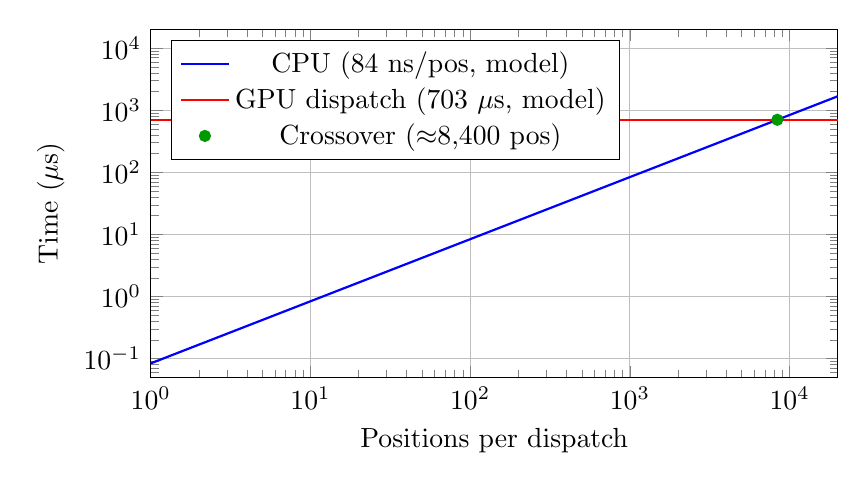
\begin{tikzpicture}
\begin{axis}[
    xlabel={Positions per dispatch},
    ylabel={Time ($\mu$s)},
    xmode=log,
    ymode=log,
    log basis x={10},
    log basis y={10},
    xmin=1, xmax=20000,
    ymin=0.05, ymax=20000,
    legend pos=north west,
    grid=major,
    width=0.85\columnwidth,
    height=6cm
]
\addplot[blue, thick, domain=1:20000] {0.084*x};
\addlegendentry{CPU (84~ns/pos, model)}
\addplot[red, thick, domain=1:20000] {703};
\addlegendentry{GPU dispatch (703~$\mu$s, model)}
\addplot[only marks, mark=*, green!60!black] coordinates {(8369, 703)};
\addlegendentry{Crossover ($\approx$8,400 pos)}
\end{axis}
\end{tikzpicture}
\caption{CPU vs GPU evaluation time under a synchronous per-dispatch model. The GPU line represents dispatch overhead, which dominates kernel compute time in our implementation; we therefore model GPU cost as constant per evaluation call. Crossover occurs at approximately 8,400 positions per dispatch.}
\label{fig:crossover}
\end{figure}

The crossover point where GPU matches CPU throughput is:
\begin{equation}
N_{\text{crossover}} = \frac{T_{\text{GPU\_dispatch}}}{T_{\text{CPU\_eval}}} = \frac{703~\mu\text{s}}{84~\text{ns}} \approx 8,369
\end{equation}

GPU acceleration only becomes beneficial when batching approximately 8,400 positions per kernel dispatch. In traditional alpha-beta search, this is impractical because:
\begin{enumerate}
\item Search is sequential: each node depends on parent's bounds
\item Pruning eliminates most nodes before evaluation
\item Speculative evaluation wastes work on pruned branches
\end{enumerate}

\subsection{Search Performance}

The engine achieves the following search performance on the standard 50-position benchmark suite at depth 13:

\begin{table}[t]
\caption{Search benchmark results (depth 13, 64MB hash, CPU evaluation)}
\label{tab:search}
\centering
\begin{tabular}{lr}
\toprule
Metric & Value \\
\midrule
Total Nodes & 2,477,446 \\
Total Time & 1,736 ms \\
Nodes/Second & 1,427,100 \\
\bottomrule
\end{tabular}
\end{table}

This NPS is achieved using CPU NNUE evaluation exclusively. The single-threaded implementation provides a baseline; production engines typically achieve higher NPS through multi-threading (Lazy SMP) and additional optimizations.

\subsection{Move Generation Verification}

Table~\ref{tab:perft} shows perft results matching established correct values.

\begin{table}[t]
\caption{Perft verification (starting position)}
\label{tab:perft}
\centering
\begin{tabular}{rr}
\toprule
Depth & Nodes \\
\midrule
1 & 20 \\
2 & 400 \\
3 & 8,902 \\
4 & 197,281 \\
5 & 4,865,609 \\
6 & 119,060,324 \\
\bottomrule
\end{tabular}
\end{table}

Additional tests verify Kiwipete (depth 5: 193,690,690), en passant, castling, and promotion positions.

\section{Discussion}

\subsection{Why GPU Acceleration Fails for Alpha-Beta}

Our measurements quantify a fundamental mismatch between GPU computing and traditional game tree search:

\textbf{Dispatch overhead dominates:} The 703~$\mu$s GPU dispatch cost includes unavoidable Metal framework operations: command buffer allocation, encoder state management, and GPU-CPU synchronization. Even with unified memory eliminating data transfer, the command buffer lifecycle imposes significant latency.

\textbf{Sequential dependencies prevent batching:} Alpha-beta search is inherently sequential---each node's evaluation affects pruning decisions for siblings. True batching would require speculative evaluation of entire subtrees, wasting computation on pruned branches.

\textbf{CPU evaluation is highly optimized:} Stockfish's NNUE implementation uses SIMD intrinsics and incremental updates, achieving sub-100~ns evaluation. GPU acceleration must overcome not just dispatch overhead but also compete with highly-tuned CPU code.

\subsection{When GPU Acceleration Helps}

GPU acceleration becomes beneficial for:
\begin{itemize}
\item \textbf{Monte Carlo Tree Search:} MCTS naturally generates large batches of leaf evaluations, amortizing dispatch overhead across hundreds of positions per dispatch~\cite{LeelaChessZero2024}
\item \textbf{Multi-position analysis:} Analyzing thousands of positions simultaneously (database analysis, puzzle solving)
\item \textbf{Training:} Neural network training requires batch processing
\item \textbf{True batched evaluation:} A single GPU dispatch evaluating multiple positions could achieve the crossover, but requires architectural changes to accumulate evaluation requests
\end{itemize}

\subsection{CPU vs GPU Evaluation Paths}

Our implementation maintains separate evaluation paths: the CPU path uses Stockfish's NNUE with fully-loaded network weights, while the GPU path uses independently-loaded weights. In our benchmarks, the GPU evaluator returns different scores than the CPU evaluator (mean difference: 46 centipawns), indicating the GPU network weights were not fully synchronized.

Critically, this weight difference does not affect our latency measurements. The GPU path executes identical kernels regardless of weight values: feature transformation (1,024-dimensional accumulator computation) and forward pass (FC0$\rightarrow$FC1$\rightarrow$FC2). The measured 703~$\mu$s dispatch overhead reflects the Metal command buffer lifecycle, not computation time, which is negligible relative to dispatch overhead. Our latency results are therefore representative of any NNUE-style GPU evaluation with the same network architecture.

\subsection{Limitations}

\begin{itemize}
\item Single-threaded search; Lazy SMP would increase CPU throughput
\item GPU path uses separate weight loading, not synchronized with CPU NNUE
\item No kernel-level batching implemented (each position dispatches separately)
\item Measurements on single hardware configuration (M2 Max)
\end{itemize}

\section{Related Work}

Leela Chess Zero~\cite{LeelaChessZero2024} pioneered GPU-accelerated MCTS for chess, demonstrating that batch-oriented search algorithms map efficiently to GPUs with batch sizes of 64--256 positions per dispatch. AlphaZero~\cite{Silver2017} showed that neural network evaluation can replace traditional handcrafted evaluation when combined with MCTS.

For alpha-beta search, prior work has explored GPU parallelization through parallel subtree evaluation~\cite{Rocki2010} and speculative execution strategies. Rocki and Suda demonstrated GPU-accelerated game tree search for simpler games, but found that communication overhead between CPU and GPU limited speedup for complex evaluation functions. Our work provides concrete measurements on modern unified memory hardware showing why single-position GPU evaluation remains counterproductive for sequential search, even when data transfer overhead is eliminated.

\section{Conclusion}

MetalFish demonstrates that GPU acceleration for chess engines requires careful consideration of dispatch overhead. Key findings:

\begin{enumerate}
\item GPU dispatch overhead (703~$\mu$s median blocking latency) exceeds CPU evaluation time (84~ns median) by 8,400$\times$ for single positions
\item Crossover requires batching approximately 8,400 positions per dispatch
\item Traditional alpha-beta search cannot exploit GPU parallelism due to sequential dependencies
\item Unified memory eliminates data transfer overhead but not dispatch overhead
\item CPU-based evaluation achieves 1.43M nodes/second in our single-threaded implementation
\end{enumerate}

These findings suggest that GPU acceleration for chess engines is most effective when combined with batch-oriented search algorithms (MCTS) or true multi-position batching within a single dispatch, rather than traditional alpha-beta search where each position requires immediate evaluation.

\subsection*{Reproducibility}

Hardware: Apple M2 Max, 64GB unified memory. Software: macOS 14.0, Xcode 15.0, Metal feature set macOS-GPUFamily2-v1. Source code: \url{https://github.com/NripeshN/MetalFish}. NNUE networks: nn-c288c895ea92.nnue (125MB), nn-37f18f62d772.nnue (6MB).

\section*{Acknowledgments}

Thanks to the Stockfish and Leela Chess Zero teams for open-source contributions informing this work.

\begin{thebibliography}{10}

\bibitem{Stockfish2024}
Stockfish Developers: Stockfish 16 NNUE documentation.
\url{https://github.com/official-stockfish/Stockfish} (2024)

\bibitem{Nickolls2008}
Nickolls, J., Buck, I., Garland, M., Skadron, K.: Scalable parallel programming with CUDA.
Queue 6(2), 40--53 (2008)

\bibitem{Knuth1975}
Knuth, D.E., Moore, R.W.: An analysis of alpha-beta pruning.
Artificial Intelligence 6(4), 293--326 (1975)

\bibitem{Reinefeld1983}
Reinefeld, A.: An improvement to the scout tree-search algorithm.
ICCA Journal 6(4), 4--14 (1983)

\bibitem{Nasu2018}
Nasu, Y.: Efficiently updatable neural-network-based evaluation functions for computer shogi.
The 28th World Computer Shogi Championship Appeal Document (2018)

\bibitem{AppleMetal2024}
Apple Inc.: Metal Best Practices Guide.
\url{https://developer.apple.com/metal/} (2024)

\bibitem{Zobrist1970}
Zobrist, A.L.: A new hashing method with application for game playing.
Tech. Rep. 88, Computer Sciences Department, University of Wisconsin (1970)

\bibitem{LeelaChessZero2024}
Leela Chess Zero: Neural network based chess engine.
\url{https://lczero.org/} (2024)

\bibitem{Silver2017}
Silver, D., et al.: Mastering chess and shogi by self-play with a general reinforcement learning algorithm.
arXiv:1712.01815 (2017)

\bibitem{Rocki2010}
Rocki, K., Suda, R.: Parallel minimax tree searching on GPU.
In: Parallel Processing and Applied Mathematics, LNCS vol. 6067, pp. 449--456. Springer (2010)

\end{thebibliography}

\end{document}
